\let\negmedspace\undefined
\let\negthickspace\undefined
\documentclass[journal]{IEEEtran}
\usepackage[a5paper, margin=10mm, onecolumn]{geometry}
\usepackage{lmodern} % Ensure lmodern is loaded for pdflatex
\usepackage{tfrupee} % Include tfrupee package

\setlength{\headheight}{1cm} % Set the height of the header box
\setlength{\headsep}{0mm}  % Set the distance between the header box and the top of the text

\usepackage{csquotes}
\usepackage{gvv-book}
\usepackage{gvv}
\usepackage{circuitikz}
\usepackage{cite}
\usepackage{amsmath,amssymb,amsfonts,amsthm}
\usepackage{algorithmic}
\usepackage{graphicx}
\usepackage{textcomp}
\usepackage{xcolor}
\usepackage{txfonts}
\usepackage{listings}
\usepackage{enumitem}
\usepackage{mathtools}
\usepackage{gensymb}
\usepackage{comment}
\usepackage[breaklinks=true]{hyperref}
\usepackage{tkz-euclide} 
\usepackage{listings}
% \usepackage{gvv}                                        
\def\inputGnumericTable{}                                 
\usepackage[latin1]{inputenc}                                
\usepackage{color}                                            
\usepackage{array}                                            
\usepackage{longtable}                                       
\usepackage{calc}                                             
\usepackage{multirow}                                         
\usepackage{hhline}                                           
\usepackage{ifthen}                                           
\usepackage{lscape}
\usepackage{caption}
\usepackage{tikz}
\usetikzlibrary{patterns}

\bibliographystyle{IEEEtran}

\begin{document}


\begin{center}
    \textbf{\Large GATE 2016\\
    AGRICULTURAL ENGINEERING (AG)\\
    MAIN PAPER}
\end{center}


\section*{Q. 1 -- Q. 5 carry one mark each.}
\begin{enumerate}
\item 
If I were you, I \dots that laptop. It's much too expensive.

\begin{enumerate}
\begin{multicols}{2}
\item won't buy
\item shan't buy
\item wouldn't buy
\item would buy
\end{multicols}
\end{enumerate}
\hfill(GATE AG 2016)\\

\medskip

\item 
He \underline{turned a deaf ear} to my request.

What does the underlined phrasal verb mean?

\begin{enumerate}
\begin{multicols}{2}
\item ignored
\item appreciated
\item twisted
\item returned
\end{multicols}
\end{enumerate}
\hfill(GATE AG 2016)\\

\medskip

\item 
Choose the most appropriate set of words from the options given below to complete the following sentence.

\emph{\dots is a will, \dots is a way.}

\begin{enumerate}
\begin{multicols}{2}
\item Wear, there, their
\item Were, their, there
\item Where, there, there
\item Where, their, their
\end{multicols}
\end{enumerate}
\hfill(GATE AG 2016)\\

\medskip

\item 
$(x\% \text{ of } y) + (y\% \text{ of } x)$ is equivalent to \dots.

\begin{enumerate}
\begin{multicols}{2}
\item 2\% of $xy$
\item 2\% of $(xy/100)$
\item $xy$\% of 100
\item 100\% of $xy$
\end{multicols}
\end{enumerate}
\hfill(GATE AG 2016)\\

\medskip

\item 
The sum of the digits of a two digit number is 12. If the new number formed by reversing the digits is greater than the original number by 54, find the original number.

\begin{enumerate}
\begin{multicols}{4}
\item 39
\item 57
\item 66
\item 93
\end{multicols}
\end{enumerate}
\hfill(GATE AG 2016)\\

\medskip

\section*{Q. 6 -- Q. 10 carry two marks each.}

\item 
Two finance companies, P and Q, declared fixed annual rates of interest on the amounts invested with them. The rates of interest offered by these companies may differ from year to year. Year-wise annual rates of interest offered by these companies are shown by the line graph provided below.

\begin{figure}[H]
    \centering
    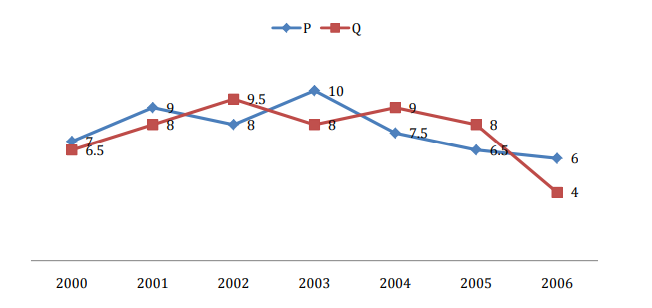
\includegraphics[width=0.5\columnwidth]{Figs/fig2.png}
    \caption{}
    \label{fig 1}
\end{figure}

If the amounts invested in the companies, P and Q, in 2006 are in the ratio 8:9, then the amounts received after one year as interests from companies P and Q would be in the ratio:
\begin{enumerate}
\begin{multicols}{4}
\item 2:3
\item 3:4
\item 6:7
\item 4:3
\end{multicols}
\end{enumerate}
\hfill(GATE AG 2016)\\

\medskip

\item 
Today, we consider Ashoka as a great ruler because of the copious evidence he left behind in the form of stone carved edicts. Historians tend to correlate greatness of a king at his time with the availability of evidence today.

Which of the following can be logically inferred from the above sentences?

\begin{enumerate}
\begin{multicols}{2}
\item Emperors who do not leave significant sculpted evidence are completely forgotten.
\item Ashoka produced stone carved edicts to ensure that later historians will respect him.
\item Statues of kings are a reminder of their greatness.
\item A king's greatness, as we know him today, is interpreted by historians.
\end{multicols}
\end{enumerate}
\hfill(GATE AG 2016)\\

\medskip

\item 
Fact 1: Humans are mammals. \\
Fact 2: Some humans are engineers. \\
Fact 3: Engineers build houses.

If the above statements are facts, which of the following can be logically inferred?

\begin{tabular}{ll}
I.    & All mammals build houses. \\
II.   & Engineers are mammals. \\
III.  & Some humans are not engineers. \\
\end{tabular}

\begin{enumerate}
\begin{multicols}{4}
\item II only.
\item III only.
\item I, II and III.
\item I only.
\end{multicols}
\end{enumerate}
\hfill(GATE AG 2016)\\

\medskip

\item 
A square pyramid has a base perimeter $x$, and the slant height is half of the perimeter. What is the lateral surface area of the pyramid?

\begin{enumerate}
\begin{multicols}{4}
\item $x^2$
\item $0.75\,x^2$
\item $0.50\,x^2$
\item $0.25\,x^2$
\end{multicols}
\end{enumerate}
\hfill(GATE AG 2016)\\

\medskip

\item 
Ananth takes 6 hours and Bharath takes 4 hours to read a book. Both started reading copies of the book at the same time. After how many hours is the number of pages to be read by Ananth, twice that to be read by Bharath? Assume Ananth and Bharath read all the pages with constant pace.

\begin{enumerate}
\begin{multicols}{4}
\item 1
\item 2
\item 3
\item 4
\end{multicols}
\end{enumerate}
\hfill(GATE AG 2016)\\

\medskip

\noindent
\textbf{GATE 2016 Agricultural Engineering (AG)}

\noindent
\textbf{Common data}\\
Acceleration due to gravity ($g$) = 9.81 m s$^{-2}$; Molecular weight of air = 28.97 kg kmol$^{-1}$; Universal gas constant = 8.314 kJ kmol$^{-1}$ K$^{-1}$.

\section*{Q. 1 -- Q. 25 carry one mark each.}

\item 
Eigen values of the matrix
$\begin{bmatrix} 5 & 3 \\ 1 & 4 \end{bmatrix}$ are
\begin{enumerate}
\begin{multicols}{2}
\item $-6.3$ and $-2.7$
\item $-2.3$ and $-6.7$
\item $6.3$ and $2.7$
\item $2.3$ and $6.7$
\end{multicols}
\end{enumerate}
\hfill(GATE AG 2016)\\

\medskip

\item 
With $n$ being a positive integer, the series $\sum_{n=1}^{\infty} \frac{1}{n^p}$, for $p > 1$ is
\begin{enumerate}
\begin{multicols}{2}
\item convergent
\item divergent
\item asymptotic
\item oscillatory
\end{multicols}
\end{enumerate}
\hfill(GATE AG 2016)\\

\medskip

\item 
The general solution of the differential equation
\begin{align}
\frac{dy}{dx} = e^{3x-2y} + x^2 e^{-2y}
\end{align}
is
\begin{enumerate}
\begin{multicols}{2}
\item $C = \frac{1}{2}e^{2y} - \frac{1}{3}(e^{3x} + x^3)$
\item $C = e^{2y} - \frac{1}{3}(e^{3x} + x^2)$
\item $C = \frac{1}{3}e^{2y} - \frac{1}{2}(e^{3x} + x^2)$
\item $C = e^{2y} - \frac{1}{3}(e^{3x} + x^3)$
\end{multicols}
\end{enumerate}
\hfill(GATE AG 2016)\\

\medskip

\item 
The function $f(x) = x^2 - x - 6$ is
\begin{enumerate}
\begin{multicols}{2}
\item minimum at $x = 1/2$
\item maximum at $x = 1/2$
\item minimum at $x = -1/2$
\item maximum at $x = -1/2$
\end{multicols}
\end{enumerate}
\hfill(GATE AG 2016)\\

\medskip

\item 
The function $f(x)$ represents a normal distribution whose standard deviation and mean are 1 and 5, respectively. The value of $f(x)$ at $x = 5$ is
\begin{enumerate}
\begin{multicols}{4}
\item 0.0
\item 0.159
\item 0.282
\item 0.398
\end{multicols}
\end{enumerate}
\hfill(GATE AG 2016)\\

\medskip

\item 
A watershed area of 1851 hectare has maximum distance of 7.12 km from the outlet to the farthest point on the divide line. The form factor of the watershed is
\begin{enumerate}
\begin{multicols}{4}
\item 2.60
\item 2.73
\item 0.365
\item 0.385
\end{multicols}
\end{enumerate}
\hfill(GATE AG 2016)\\

\medskip

\item 
The normal annual rainfall for 5 rain gauge stations A, B, C, D, and E in a watershed were 112.7, 120.4, 118.3, 125.2, and 110.6 cm, respectively. In a particular year, the rain gauge installed at station C failed to record rainfall. In the same year the rain gauges at stations A, B, D and E recorded annual rainfall of 114.9, 118.3, 122.6 and 114.5 cm, respectively. The estimated rainfall at station C in that particular year in cm was \dots
\hfill(GATE AG 2016)\\

\medskip


\item 
Annual average soil loss from a watershed has been measured as 20 Mg ha$^{-1}$ year$^{-1}$. Watershed has 8\% land slope and 84 m maximum slope length. Assume all other factors same and dimensionless exponent for slope factor is 0.5. To reduce soil loss from the watershed to 10 Mg ha$^{-1}$ year$^{-1}$, the maximum slope length in m should be \dots
\hfill(GATE AG 2016)\\

\medskip

\item 
In a cropped field, the following data are observed.\\
Moisture content at field capacity (weight basis) = 36\%\\
Current moisture content (weight basis) = 24\%\\
Bulk density of soil = 1.5 Mg m$^{-3}$\\
Effective root zone depth = 0.8 m\\
Conveyance efficiency = 80\%\\
Application efficiency = 90\%\\
To bring soil moisture content to field capacity, the depth of irrigation in mm will be \dots
\hfill(GATE AG 2016)\\

\medskip

\item 
The correct conditions for which the hydraulically efficient rectangular channel will deliver maximum discharge are

P -- depth of water is equal to half the breadth of channel\\
Q -- depth of water is equal to breadth of channel\\
R -- depth of water is equal to twice the breadth of channel\\
S -- hydraulic radius is equal to half the depth of water

\begin{enumerate}
\begin{multicols}{4}
\item P and R
\item P and Q
\item P and S
\item R and S
\end{multicols}
\end{enumerate}
\hfill(GATE AG 2016)\\

\medskip

\item 
The most suitable hydraulic structure for conveying water from higher elevation to lower elevation across the earthen bund is

\begin{enumerate}
\begin{multicols}{2}
\item Drop structure
\item Pipe drop structure
\item Chute spillway
\item Gabion structure
\end{multicols}
\end{enumerate}
\hfill(GATE AG 2016)\\

\medskip

\item 
Match the following

\begin{tabular}{ll}
(P) Waste valve          & (1) Jet pump \\
(Q) Plunger              & (2) Centrifugal pump \\
(R) Foot valve           & (3) Reciprocating pump \\
(S) Nozzle and venturi   & (4) Hydraulic ram \\
\end{tabular}

\begin{enumerate}
\begin{multicols}{2}
\item P-3, Q-2, R-4, S-1
\item P-4, Q-2, R-3, S-1
\item P-1, Q-3, R-4, S-2
\item P-4, Q-3, R-2, S-1
\end{multicols}
\end{enumerate}
\hfill(GATE AG 2016)\\

\medskip

\item 
The ASAE-SAE standard for tractor 3-point hitches has been categorized as Category I to IV on the basis of

\begin{enumerate}
\begin{multicols}{2}
\item maximum drawbar power
\item maximum drawbar pull
\item brake power of tractor engine
\item maximum PTO power
\end{multicols}
\end{enumerate}
\hfill(GATE AG 2016)\\

\medskip

\noindent
\textbf{GATE 2016 Agricultural Engineering (AG)}

\item 
A force of 8.0 kN is applied perpendicularly to the axis of a crankpin having circular cross-sectional area. The allowable shear stress of the crankpin material is 40.0 N mm$^{-2}$. If the crankpin fails under double shear, the design diameter of the crankpin in mm is \dots
\hfill(GATE AG 2016)\\

\medskip

\item 
A vertical rotor planter has 8 cells on each rotor. The rolling radius of the ground wheel is 200 mm. The ratio of rpm of the ground wheel to that of the rotor shaft is 2:3. If the planting is done at a forward speed of 3.5 km h$^{-1}$, the plant spacing in the rows in mm will be \dots.
\hfill(GATE AG 2016)\\

\medskip

\item 
The effective temperature (ET) scale developed in 1972 on the basis of a human model is
\begin{enumerate}
\begin{multicols}{2}
\item Heart rate
\item Blood pressure
\item Psychological response
\item Physiological response
\end{multicols}
\end{enumerate}
\hfill(GATE AG 2016)\\

\medskip

\item 
As per ASAE standards, the diameter of 1000 rpm-PTO shaft with 20 splines is
\begin{enumerate}
\begin{multicols}{4}
\item 30 mm
\item 35 mm
\item 40 mm
\item 45 mm
\end{multicols}
\end{enumerate}
\hfill(GATE AG 2016)\\

\medskip

\item 
In restrained link operation of three point hitches, the line of pull passes
\begin{enumerate}
\begin{multicols}{2}
\item through the virtual hitch point and bending force exists on lower links
\item above the virtual hitch point and bending force exists on lower links
\item below the virtual hitch point and no bending force exists on lower links
\item through the virtual hitch point and tensile force exists on lower links
\end{multicols}
\end{enumerate}
\hfill(GATE AG 2016)\\

\medskip

\item 
A gear pump discharges 100 L min$^{-1}$ against a system pressure of 15 MPa. The overall efficiency of the pump is 0.75. Input power to run the pump in kW is \dots.
\hfill(GATE AG 2016)\\

\medskip

\item 
A 2.5 m long pipe is insulated at both ends. It has ID and OD as 50 mm and 56 mm, respectively. Its log-mean heat transfer area in m$^2$ is \dots.
\hfill(GATE AG 2016)\\

\medskip

\item 
In a drying experiment, the constant rate of drying is found to be 3.6 kg water m$^{-2}$ h$^{-1}$. Dry bulb and wet bulb temperatures of the drying air are 75$^\circ$C and 37$^\circ$C, respectively. Latent heats of vaporization at the dry bulb and the wet bulb temperatures are 2321 and 2414 kJ kg$^{-1}$, respectively. Convective heat transfer coefficient in W m$^{-2}$ K$^{-1}$ for the drying operation is \dots.
\hfill(GATE AG 2016)\\

\medskip

\item 
An air--water vapour mixture is at 35$^\circ$C and normal atmospheric pressure with absolute humidity of 0.02 kg water vapour kg$^{-1}$ dry air. Its humid volume in m$^3$ kg$^{-1}$ dry air is \dots.
\hfill(GATE AG 2016)\\

\medskip

\noindent
\textbf{GATE 2016 Agricultural Engineering (AG)}

\item 
A very small particle of diameter $d_p$ and density $\rho_p$ freely settles at constant velocity in a tank of depth $L$ containing liquid of viscosity $\mu_l$. The density of the liquid is $\rho_l$ where $\rho_l < \rho_p$. The velocity of particle in the liquid can be expressed as
\begin{enumerate}
\begin{multicols}{2}
\item $\displaystyle \frac{g L (\rho_p - \rho_l) d_p}{18 \mu_l}$
\item $\displaystyle \frac{g (\rho_p - \rho_l) d_p^3}{18 L \mu_l}$
\item $\displaystyle \frac{g (\rho_p - \rho_l) d_p^2}{18 \mu_l}$
\item $\displaystyle \frac{g (\rho_p - \rho_l) L^2}{18 \mu_l}$
\end{multicols}
\end{enumerate}
\hfill(GATE AG 2016)\\

\medskip

\item 
A high speed tubular ultracentrifuge with bowl radius of 100 mm and height 500 mm rotates at 20000 rpm and settles starch particles (average diameter of 20$\mu$m) on the wall. The ratio of centrifugal force to the gravitational force acting on the particle is \dots.
\hfill(GATE AG 2016)\\

\item Match the following

\begin{tabular}{ll}
(P) Wheat milling     & (1) Rubber rolls \\
(Q) Paddy dehusking  & (2) Abrasive emery roll cylinder \\
(R) Pulse dehusking  & (3) Break and reduction rolls \\
(S) Spice grinding   & (4) Hammer mills \\
\end{tabular}

\begin{enumerate}
\begin{multicols}{2}
\item P-2, Q-1, R-3, S-4
\item P-1, Q-2, R-4, S-3
\item P-3, Q-1, R-2, S-4
\item P-1, Q-3, R-4, S-2
\end{multicols}
\end{enumerate}
\hfill(GATE AG 2016)\\

\medskip

\section*{Q. 26 -- Q. 55 carry two marks each.}

\item 
Integration by trapezoidal method of $\log_{10}(x)$ with lower limit of $1$ to upper limit of $3$ using seven distinct values (equally covering the whole range) is \dots
\hfill(GATE AG 2016)\\

\medskip

\item 
The value of the integral, $I = \int_{2}^{4} \frac{x^2+1}{x^2-1}dx$ is \dots
\hfill(GATE AG 2016)\\

\medskip

\item 
Let $\mathbf{I}$, $\mathbf{J}$, and $\mathbf{K}$ are unit vectors along the three mutually perpendicular $x$, $y$ and $z$ axes, respectively. If $\mathbf{F} = f\mathbf{I} + g\mathbf{J} + h\mathbf{K}$ is a continuously differentiable vector point function, then $\mathbf{curl\ F}$ is
\begin{enumerate}
\begin{multicols}{2}
\item $\mathbf{I}\left( \dfrac{\partial g}{\partial z} - \dfrac{\partial h}{\partial y} \right ) - \mathbf{J} \left ( \dfrac{\partial f}{\partial x} - \dfrac{\partial h}{\partial x} \right) + \mathbf{K} \left( \dfrac{\partial f}{\partial y} - \dfrac{\partial g}{\partial x} \right )$
\item $\mathbf{I}\left( \dfrac{\partial h}{\partial y} - \dfrac{\partial g}{\partial z} \right ) - \mathbf{J} \left ( \dfrac{\partial h}{\partial x} - \dfrac{\partial f}{\partial z} \right) + \mathbf{K} \left( \dfrac{\partial g}{\partial x} - \dfrac{\partial f}{\partial y} \right )$
\item $\mathbf{I}\left( \dfrac{\partial h}{\partial y} - \dfrac{\partial g}{\partial z} \right ) + \mathbf{J} \left ( \dfrac{\partial h}{\partial x} - \dfrac{\partial f}{\partial z} \right) + \mathbf{K} \left( \dfrac{\partial g}{\partial x} - \dfrac{\partial f}{\partial y} \right )$
\item $\mathbf{I}\left( \dfrac{\partial g}{\partial z} - \dfrac{\partial h}{\partial y} \right ) + \mathbf{J} \left ( \dfrac{\partial f}{\partial z} - \dfrac{\partial h}{\partial x} \right) + \mathbf{K} \left( \dfrac{\partial f}{\partial y} - \dfrac{\partial g}{\partial x} \right )$
\end{multicols}
\end{enumerate}
\hfill(GATE AG 2016)\\

\medskip

\noindent
\textbf{GATE 2016 Agricultural Engineering (AG)}

\item 
The maximum one day rainfall depth at 20 year return period of a city is 150 mm. The probability of one day rainfall equal to or greater than 150 mm in the same city occurring twice in 20 successive years is \dots.
\hfill(GATE AG 2016)\\

\medskip

\item 
The back sight of 1.258 m was observed for the bench mark (BM) at reduced level (RL) of 48 m. The corresponding fore sight on the staff held vertically inverted to the underside of a bridge beam is 4.645 m. The RL at the underside of the bridge beam in m is
\begin{enumerate}
\begin{multicols}{4}
\item 44.613
\item 46.936
\item 51.581
\item 53.903
\end{multicols}
\end{enumerate}
\hfill(GATE AG 2016)\\

\medskip

\item 
The observed rainfall of a 12 h duration event is given in the table below. If the phi ($\Phi$) index of the storm is 0.46, the total direct runoff of the event in mm will be \dots.
\hfill(GATE AG 2016)\\

\medskip

\begin{center}
\begin{tabular}{| m{3cm} | m{3cm} |}
\hline
\textbf{Macronutrient} & \textbf{Energy density (kcal/g)} \\
\hline
Carbohydrates & 4 \\
Proteins & 4 \\
Unsaturated fat & 9 \\
Saturated fat & 9 \\
Trans fat & 9 \\
\hline
\end{tabular}
\end{center}

\medskip

\item 
If the width of bench terrace is $W$, drop $D$ and existing land slope $S$; then for 150\% batter slope, the drop D will be
\begin{enumerate}
\begin{multicols}{4}
\item $\dfrac{WS}{100}$
\item $\dfrac{WS}{100-5}$
\item $\dfrac{2WS}{200-5}$
\item $\dfrac{3WS}{300-2.5}$
\end{multicols}
\end{enumerate}
\hfill(GATE AG 2016)\\

\medskip

\item 
A 3 m high retaining wall supports sandy soil of unit weight 18.5 kN m$^{-3}$. The angle of shearing resistance ($\phi$) is $30^\circ$ and the surface of soil is horizontal. The magnitude of the active thrust (in kN m$^{-1}$) and its acting point from the top (in m) are
\begin{enumerate}
\begin{multicols}{2}
\item 27.75 and 1
\item 249.75 and 1
\item 27.75 and 2
\item 249.75 and 2
\end{multicols}
\end{enumerate}
\hfill(GATE AG 2016)\\

\medskip

\item 
A soil has bulk density and particle density of 1.48 Mg m$^{-3}$ and 2.64 Mg m$^{-3}$, respectively. The saturated volumetric moisture content of soil is 36\%. The porosity and void ratio of the soil are
\begin{enumerate}
\begin{multicols}{2}
\item 0.36 and 0.56
\item 0.44 and 0.79
\item 0.79 and 0.44
\item 0.56 and 0.36
\end{multicols}
\end{enumerate}
\hfill(GATE AG 2016)\\

\medskip

\item 
A solid set permanent micro-irrigation system is installed in a vegetable field of 1 ha area. The spacing between the micro sprinklers is 2.5 m and spacing between laterals is 5 m. The peak evapotranspiration rate is 10 mm day$^{-1}$. The application efficiency is 80\%. Irrigation system operates 5 hours in a day. The total operating head of the pump is 30 m. At 65\% pump efficiency, the horse power of the pump is \dots.
\hfill(GATE AG 2016)\\

\medskip

\item 
The discharge of a centrifugal pump is 25 L s$^{-1}$ against the delivery head of 10 m. The outlet of the delivery pipe is submerged. A 200 m long 100 mm diameter pipe is connected with the delivery end of the pump. The friction factor for the pipe is 0.03. The minor losses in the delivery pipe are 1 m. The pressure at the delivery end of the pump in kPa is \dots.
\hfill(GATE AG 2016)\\

\medskip


\noindent
\textbf{GATE 2016 Agricultural Engineering (AG)}

\item 
In a subsurface drainage system, the peak discharge through tile drain under full flow condition is given by
\[
Q = 6.715 \times 10^{-4} S^{0.5} n^{-1}
\]
where, $Q =$ discharge, m$^3$ s$^{-1}$, $S =$ drain bed slope and $n =$ Manning's roughness coefficient. Size of the drain in mm is \dots.
\hfill(GATE AG 2016)\\

\medskip

\item 
A fully penetrating tube well in a 30 m deep confined aquifer with hydraulic conductivity of $4\times 10^{-4}$ m s$^{-1}$ has 50 L s$^{-1}$ discharge. The drawdown and radius of influence are 5 m and 250 m, respectively. Diameter of the tube well in mm is \dots.
\hfill(GATE AG 2016)\\

\medskip

\item 
An inclined blade cutting tool of 250 mm width is operating at 200 mm cutting depth. The normal load on the tool and the coefficient of soil-metal friction are 1000 N and 0.3, respectively. The soil cutting force per unit length of cutting edge is 20 N mm$^{-1}$. The tool lift angle is $40^\circ$. The required specific draft (or unit draft) in kPa is \dots.
\hfill(GATE AG 2016)\\

\medskip

\item 
The rated nozzle flow rate and volume median diameter (VMD) of droplets of a hydraulic sprayer are 1.0 L min$^{-1}$ and 200 $\mu$m, respectively at the rated pressure of 500 kPa. If the desired nozzle flow rate is 1.5 L min$^{-1}$, the droplet diameter in $\mu$m will be \dots.
\hfill(GATE AG 2016)\\

\medskip

\item 
A water pumping system is being driven by a propeller type wind turbine having the power coefficient of 0.4. The total pumping head and rate of discharge are 20 m and 7.0 L s$^{-1}$, respectively. Mean wind velocity is 18 km h$^{-1}$ and the density of air is 1.2 kg m$^{-3}$. The required diameter of the propeller in m is \dots.
\hfill(GATE AG 2016)\\

\medskip

\item 
While testing a wheat thresher at the recommended throughput, 80 N m torque is recorded at 750 rpm at the main shaft of the threshing cylinder, which is operated by a 200 mm diameter v-pulley. The overload factor and unit mass of the v-belt are 1.2 and 0.9 kg m$^{-1}$, respectively. At the condition of maximum power transmission, the maximum tension in the v-belt in N is \dots.
\hfill(GATE AG 2016)\\

\medskip

\item 
A tractor PTO operated 4-disc rotary mower is harvesting with a forward speed of 3.5 km h$^{-1}$. The cutting circle diameter and rpm of each disc are 60 cm and 1400, respectively. The peak cutting force experienced by each rotary disc is 110 N. The peak overall motion resistance is found to be 3.6 kN. If the overall power conversion efficiency of the tractor is 82\%, required peak engine brake power in kW will be \dots.
\hfill(GATE AG 2016)\\

\medskip

\noindent
\textbf{GATE 2016 Agricultural Engineering (AG)}

\item 
Natural frequency of an undamped operator seat is 5 Hz, and combined weight of the seat and the operator is 880 N. If there are four springs fitted in parallel below the operator seat, the spring rate (or stiffness) of each spring in kN m$^{-1}$ is \dots.
\hfill(GATE AG 2016)\\

\medskip

\item
The intake pressure of a diesel engine is 1 bar and pressure at the end of the compression is 34 bar. The adiabatic exponent is 1.3 and the expansion ratio is 7. The diesel cycle efficiency in percentage is \dots.
\hfill(GATE AG 2016)\\

\medskip

\item 
In a tractor rear axle differential, the bevel pinion has 12 teeth and bevel/crown gear has 42 teeth. The input speed and torque of the bevel pinion are 520 rpm and 1200 N m, respectively. There is a planetary gear between the differential unit and each half axle with 4:1 speed reduction. The left wheel encounters poor traction when the tractor is moving in straight path that causes 15\% drop in the left axle torque. If the differential efficiency is 0.98, the right axle torque under locked differential condition in N m will be \dots.
\hfill(GATE AG 2016)\\

\medskip

\item 
A tractor weighing 21 kN has 70\% static weight on rear axle and its wheel base is 1.8 m. The drawbar hitch is located 25 cm behind the rear axle centre and 35 cm above the ground level. To overcome longitudinal instability, the front end loading is provided at a distance of 20 cm ahead of the front axle centre. It is observed that, there is front-end instability in the tractor due to a pull of 30 kN inclined at 20$^\circ$ downward from the horizontal. A minimum front-end load required to overcome the instability in N is \dots.
\hfill(GATE AG 2016)\\

\medskip

\item 
A gasifier uses rice husk as fuel and generates producer gas containing CO - 23\%, CO$_2$ - 4.4\%, O$_2$ - 2.6\% and N$_2$ - 70\%; all expressed in mole\%. Atomic mass of C, O and N are 12, 16 and 14, respectively. Average molecular weight of the producer gas in kg kmol$^{-1}$ is \dots.
\hfill(GATE AG 2016)\\

\medskip

\item 
One hundred kilogram spice is extracted for essential oil using twice the amount of a pure organic solvent. The extracted solid mass contains 5\% residual oil (oil-free solid mass basis). The liquid extracted mass contains 20\% oil. Assume no solvent is retained by the extracted solid mass. Initial mass of the oil in the spice in kg is \dots.
\hfill(GATE AG 2016)\\


\medskip

\item 
Milk sterilization kinetics is based on inactivation of index microorganism, \textit{Bacillus stearothermophilus}. The D-values at 121.1$^\circ$C and 139.1$^\circ$C are 1.2 min and 0.019 min, respectively. For 12 log-cycle reduction of this microorganism at 130$^\circ$C, the processing time in second is \dots.
\hfill(GATE AG 2016)\\

\textbf{GATE 2016 Agricultural Engineering (AG)}

\item
A circular grain silo with conical bottom, as shown in figure, is filled with wheat (true density 1200 kg m$^{-3}$) with porosity of 0.6. Five hundred metric tonne of wheat fills 80\% of its capacity (by volume). The total height ($h$) of the silo from its grain outlet end in m is \rule{3cm}{0.15mm}.
\begin{figure}[H]
    \centering
    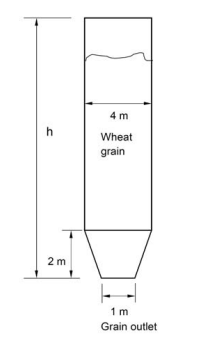
\includegraphics[width=0.4\columnwidth]{Figs/fig1.png}
    \caption{}
    \label{fig 2}
\end{figure}
\hfill(GATE AG 2016)\\


\medskip

\item 
View factor of a large cylinder of 10 cm in radius and 60 cm in length from a coaxial smaller cylinder of 5 cm radius and the same length is 0.34. View factor of the larger cylinder of itself (concave inner surface) is 0.25. The view factor of the larger cylinder with respect to either annular end is
\begin{enumerate}
\begin{multicols}{4}
\item 0.17
\item 0.29
\item 0.33
\item 0.42
\end{multicols}
\end{enumerate}
\hfill(GATE AG 2016)\\


\medskip

\item 
Mass transfer coefficient for equimolar counter-diffusion of water vapour in air is 0.4 m s$^{-1}$ (based on concentration difference). Mass diffusivity of water vapour in air is $3 \times 10^{-4}$ m$^2$ s$^{-1}$. For 100 $\mu$m diameter droplet, the Sherwood Number ($N_{sh}$) is equal to
\begin{enumerate}
\begin{multicols}{2}
\item the mass transfer coefficient
\item diameter divided by mass diffusivity
\item one - third of the mass transfer coefficient
\item three times of the mass diffusivity
\end{multicols}
\end{enumerate}
\hfill(GATE AG 2016)\\


\medskip

\item 
Hot water at 95$^\circ$C is used in a plate heat exchanger for heating 2 kg s$^{-1}$ fruit juice from 45$^\circ$C to 75$^\circ$C. Specific heat capacity of fruit juice is 3.7 kJ kg$^{-1}$ K$^{-1}$. Final temperature of the hot water is 70$^\circ$C. Overall heat transfer coefficient is 1122 W m$^{-2}$K$^{-1}$. Heat transfer area is 12.75 m$^2$. The log-mean temperature correction factor is \dots.
\hfill(GATE AG 2016)\\


\item 
In a particle size analysis, the following results are obtained:

\begin{tabular}{llcll}
\textbf{Technique} & & & \textbf{Purpose} \\[6pt]
P \; Mulching        & & & 1 \; Dust control \\
Q \; Aeration        & & & 2 \; Noise control \\
R \; Wet-scrubbing   & & & 3 \; Soil conservation \\
S \; Silencer        & & & 4 \; Waste water treatment \\
\end{tabular}

Volume-surface mean diameter of the particles in $\mu$m is \dots.
\hfill(GATE AG 2016)\\


\begin{center}
\textbf{END OF THE QUESTION PAPER}
\end{center}

\end{enumerate}

\end{document}

